\chapter{Methodology}

\par
In order to test the proposed solution, a digital twin of the oil cycle is created with a process composed of three parts. Matlab/Simulink software is selected to model the system. For modeling, mathematical equations\cite{gasomi} and experimental results are used. The experiment was done in 2022 by Ertugrul Altun for his thesis given in \cite{altun}. 
\par
First, the governing equations, which are derived in the previous chapter, are used to create a Simulink model. All variables are determined, and missing values are calculated from experimental data by curve fitting. Secondly, free variables are fitted to the experimental data with a manual training process. Finally, the model is validated by experimental data that is reserved only for validation.
\par
Free variables:
\begin{itemize}
    \item $UA$
    \item $m_{r}c_{r}$
    \item $Q_{loss}$
\end{itemize}

\section{Modeling}

The system is composed of four main components:

\begin{enumerate}
    \item Heater 
    \item Pump
    \item Evaporator
    \item Tank
\end{enumerate}

\par
Each component has a governing differential equation that needs to be solved to give the current temperature. Therefore three differential equations are defined in three subsystems with Simulink blocks for each component. The differential equation for the pump is not defined since the pump has no effect on the oil properties. It only enables the continuity of the flow. 

\par
The volumetric flow rate is taken as constant through the entire system and for all temperatures because it barely changes through desired temperature change and for each component if the outliers are neglected. This can be seen in Figure \ref{fig:volumetric}.

\begin{figure}[h]
    \centering
    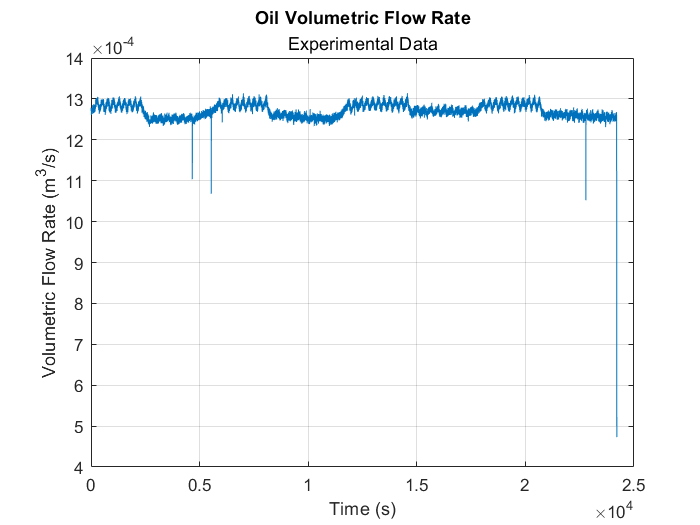
\includegraphics[width=10cm]{images/flowrate.png}
    \caption{Oil's volumetric flow rate during the experiment.}
    \label{fig:volumetric}
\end{figure}

\par
Volumetric flow rate is equal to $v = 0.001278 m^3/s$.

\par
Below assumptions are made to solve the system:
\begin{itemize}
    \item For all components, the temperature inside the component is assumed to be equal to the temperature at the exit of that component.
    \item Total heat loss in the system is assumed to be lost at the tank.
\end{itemize}

\subsection{Heater}
The heater is the place where the oil temperature is controlled. There is a thermostat that provides an interface for users to set the desired temperature. Then, the heater heats the oil up to the desired temperature. It uses an on-off temperature control unit supplying electrical power to a resistor. This resistor then transfers heat to the flowing oil.
\par
Because of two main reasons, oscillation occurs in the temperature of the oil. One is that this system is highly dependent on the measured oil temperature in the heater, and there is a hysteresis of 2.6  $^\circ$C in the thermocouple that measures the oil's temperature. This creates a lag between the real temperature and the readings. The second reason is the thermal energy storage of resistors. Because the temperature control unit only can be fully open or closed, resistors are always at different temperatures than the oil. Thus, when the heater is turned off, resistors are still hot enough to increase the oil's temperature further above the desired level. Heater parameters are provided in Table \ref{tab:heater}.

\begin{table}[h]
    \centering
    \caption{Heater parameters.}
    \label{tab:heater}
    \begin{tabular}{|c|c|c|}
        \hline
        \textbf{Symbol} & \textbf{Property}                         & \textbf{Unit} \\
        \hline
        $T_{2}$         & Oil temperature in heater                 & Kelvin \\
        $m_{2}$         & Oil mass in heater                        & kg \\
        $c_{2}$         & Oil's specific heat in heater             & kJ/kg*K \\
        $Q$             & Heat transferred to oil from resistor     & kJ \\
        $W$             & Electrical work input                     & kW \\
        $\dot{m_{1}}$   & Oil mass flow rate at heater enterence    & kg/s \\
        $\dot{m_{2}}$   & Oil mass flow rate at heater exit         & kg/s \\
        $h_{1}$         & Oil enthalpy at heater enterence          & kJ/kg \\
        $h_{2}$         & Oil enthalpy at heater exit               & kJ/kg \\
        $U$             & Resistor overall heat transfer coefficient & W/m$^2$K \\
        $A$             & Resistor surface area                     & m$^2$ \\
        $T_{r}$         & Resistor temperature                      & Kelvin \\
        $m_{r}$         & Resistor mass                             & kg \\
        $c_{r}$         & Resistor specific heat                    & kJ/kg*K \\
        \hline
    \end{tabular}
\end{table}

\par
Equation \ref*{eqn:heater} represents the governing differential equation for the heater. Every parameter in that equation needs to be found to achieve a solution. 

\begin{equation}
    \label{eqn:heater}
    \frac{dT_{2}}{dt} = \frac{1}{m_{2}c_{2}}(Q + \dot{m_{1}}h_{1} - \dot{m_{2}}h_{2})
\end{equation}

\par
For representation purposes, the heater model created in Simulink is provided in Figure \ref{fig:heater}. The controller decides if the power will be provided to the resistor. Resistor's temperature is determined by its governing differential equation, which is the combination of Equation \ref{eqn:Q} and \ref{eqn:R}. Further detail can be investigated in the appendix section (See Appendix \ref{appa}).

\begin{figure}[h]
    \centering
    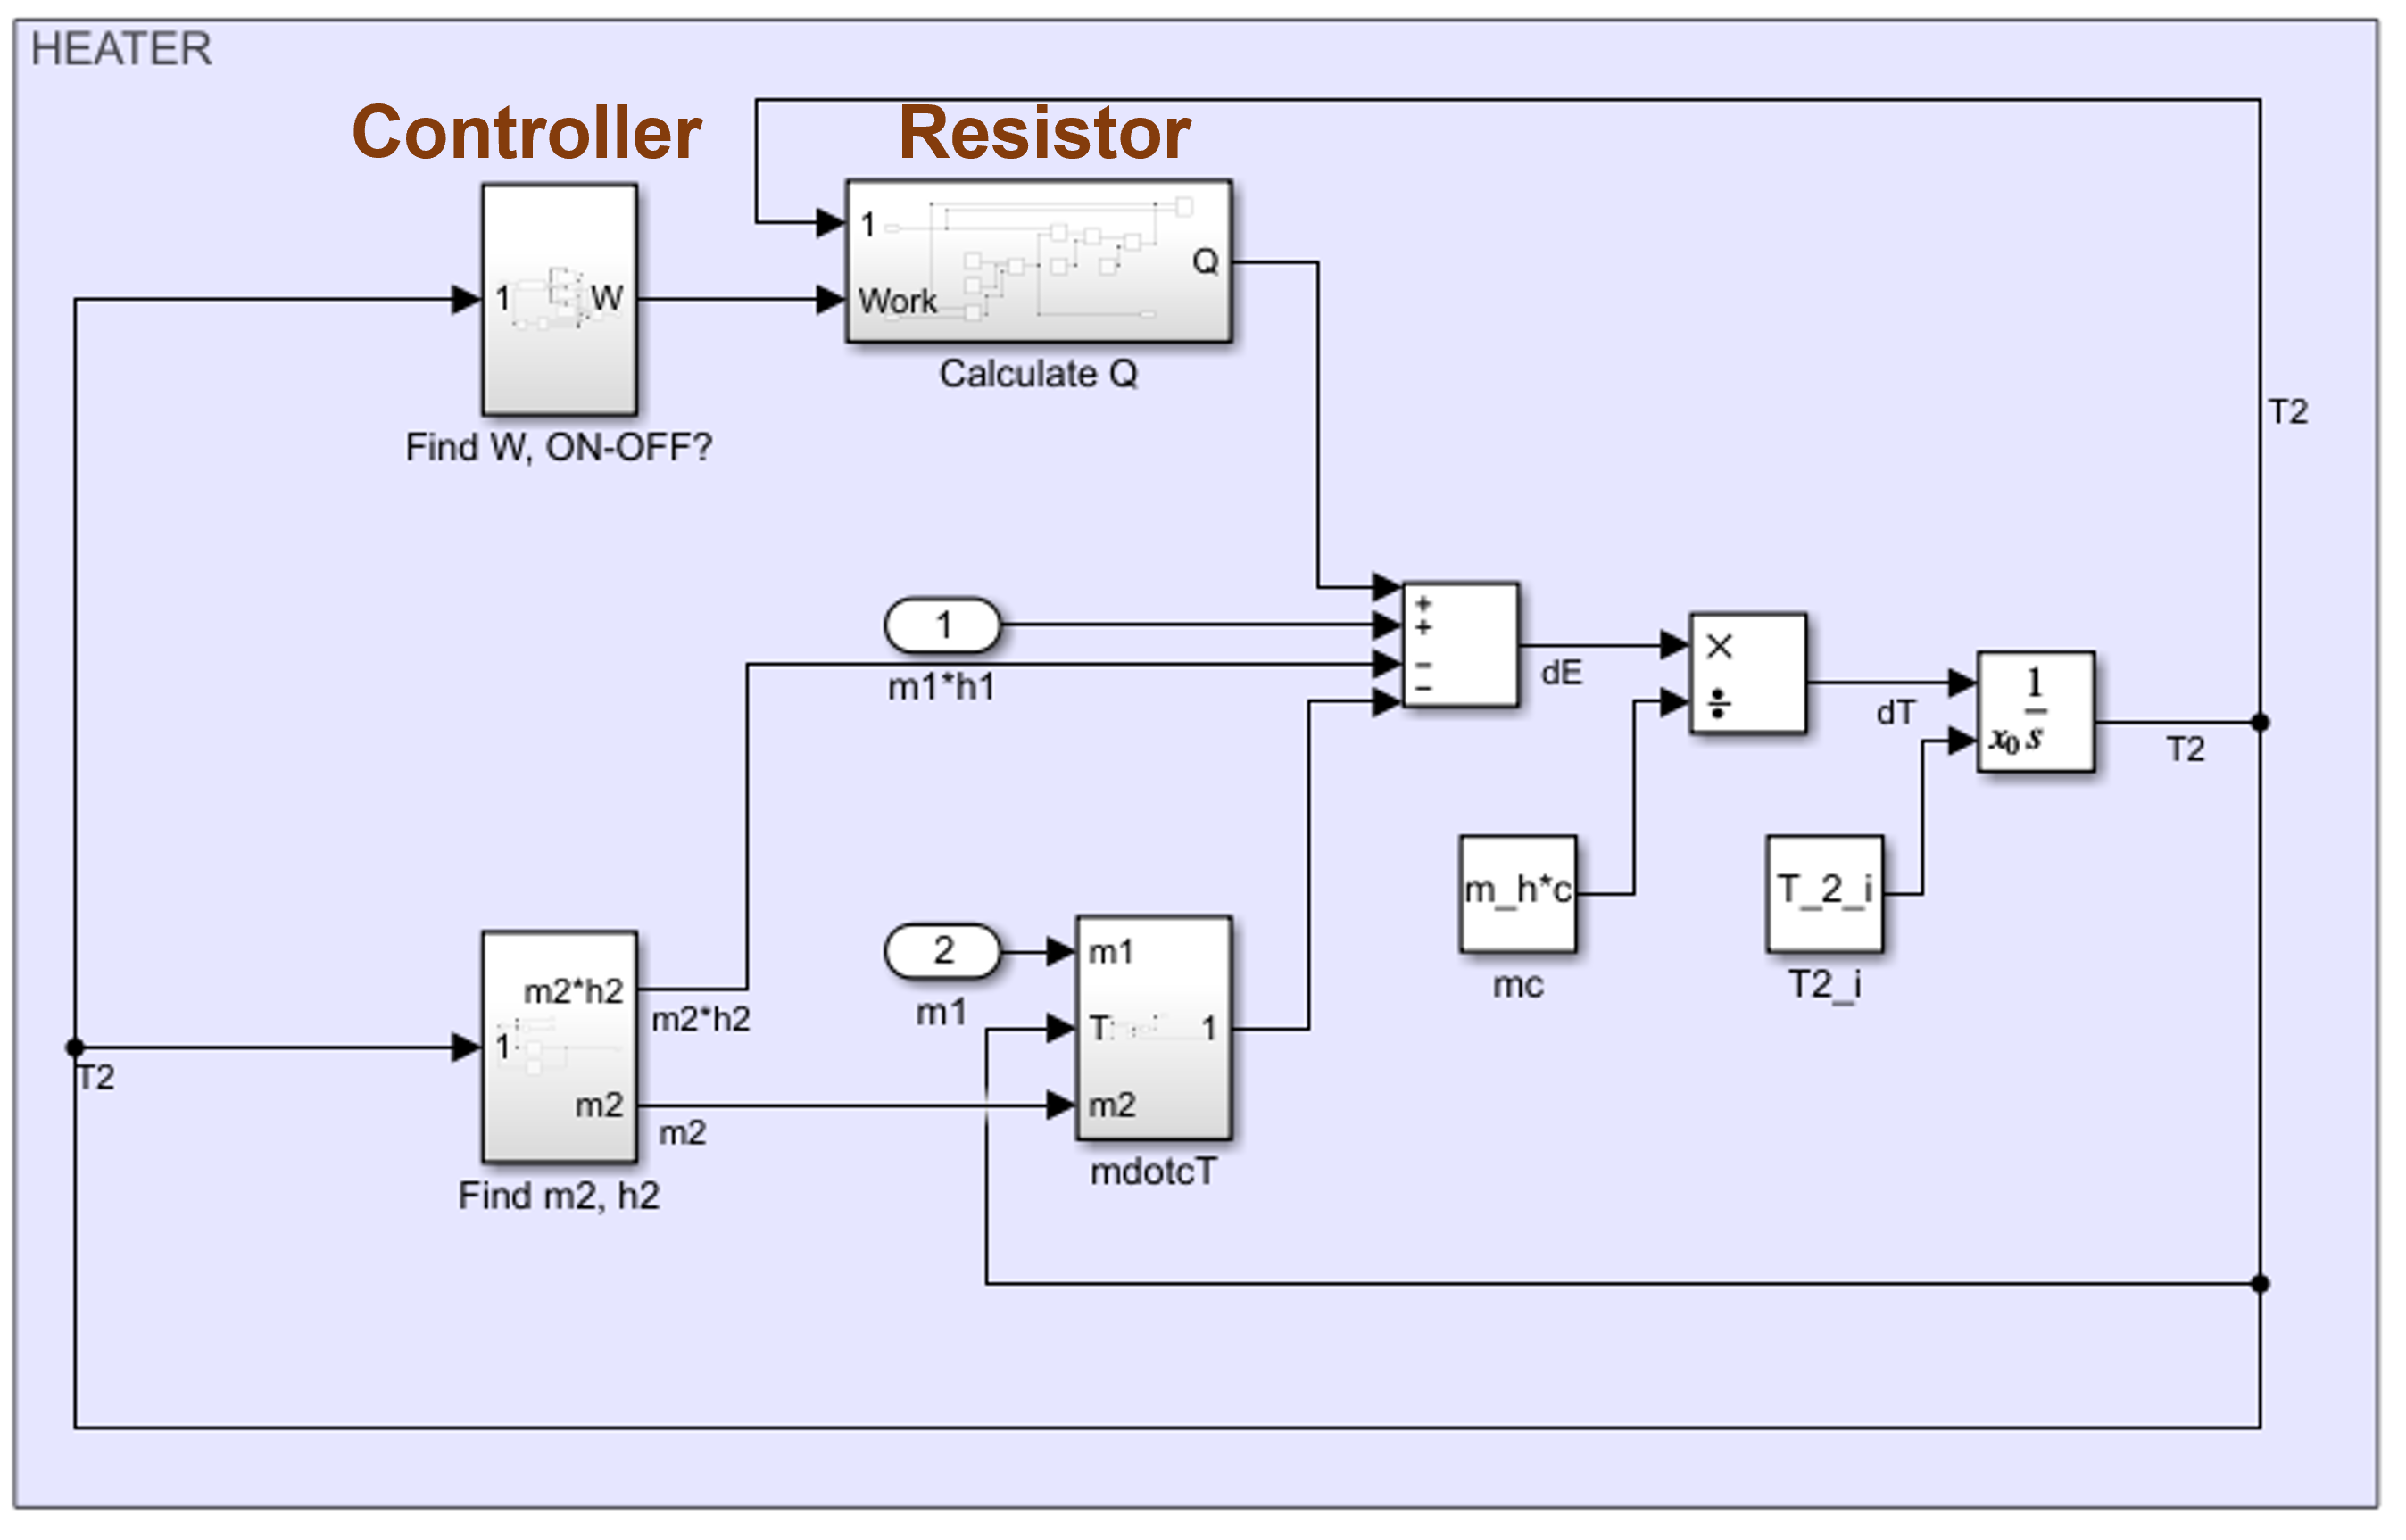
\includegraphics[width=12cm]{images/heater.png}
    \caption{Heater Simulink model.}
    \label{fig:heater}
\end{figure}

\par
In order to calculate the mass flow rate and mass ($\dot{m_{2}}$ and $m_{2}$) inside the heater, volume, and density are required according to Equations \ref{eqn:mass} and \ref{eqn:massflow}. 

\begin{equation}
    \label{eqn:massflow}
    \dot{m} = \rho * \upsilon
\end{equation}
\begin{equation}
    \label{eqn:mass}
    m= \rho * V
\end{equation}

\par
The approximate value of the heater's volume is calculated by on-site measurements and it is equal to $v_{h} = 0.29 m^2$. The density of the oil changes according to the instant temperature. To account for this change, a lookup table is entered into the Simulink model, which determines the density of the oil and makes linear interpolation if necessary. Specific heat ($c_{2}$) and enthalpy values ($h_{1}$ and $h_{2}$) are also determined by a lookup table since it also changes with temperature. These tables are provided in Figure \ref{fig:lookup}.

\begin{figure}[h]
    \begin{minipage}{.5\textwidth}
        \centering
        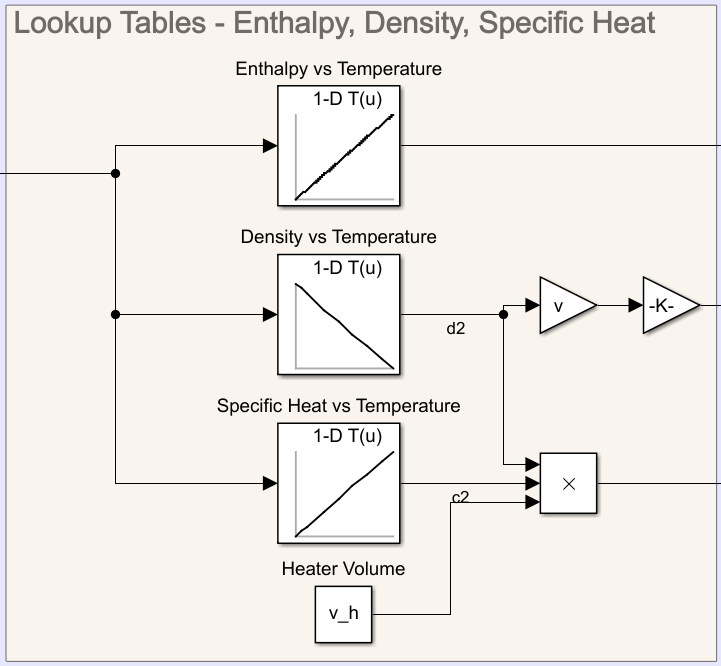
\includegraphics[width=6cm]{images/lookup.png}
        \captionof{figure}{Lookup tables Simulink model.}
        \label{fig:lookup}
    \end{minipage}
    \begin{minipage}{.4\textwidth}
        \centering
        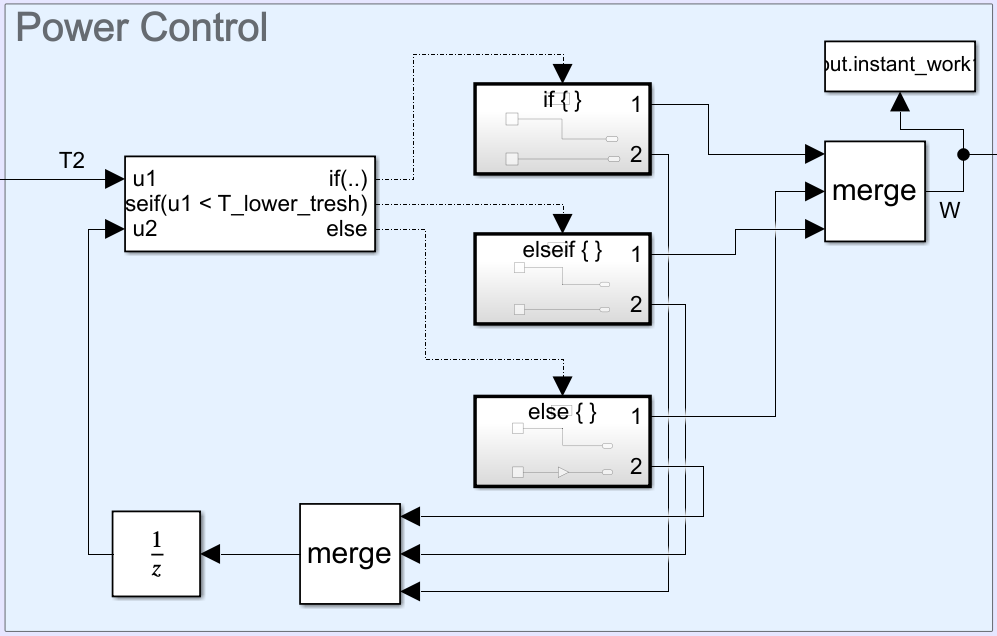
\includegraphics[width=7cm]{images/power.png}
        \captionof{figure}{Power control Simulink model.}
        \label{fig:power}
    \end{minipage}
\end{figure}

\par
Heat transferred to the oil ($Q$) is determined by carrying out the heat transfer calculations between the resistor and oil. 100 kW of electrical power is given to the resistor causing it to dissipate heat. Heat transfer\cite{incropera} to the oil from the resistor is calculated by Equation \ref{eqn:Q}.

\begin{equation}
    \label{eqn:Q}
    Q = UA(T_{r} - T_{2})
\end{equation}

\begin{equation}
    \label{eqn:R}
    \frac{dT_{r}}{dt} = \frac{1}{m_{r}c_{r}}(W - Q) 
\end{equation}

\par
Resistor's temperature ($T_{r}$) is obtained by solving the differential equation given by Equation \ref{eqn:R}. In this equation, the value of the power changes from 0 to 100 kW according to the state of the controller. When the temperature of the oil at the heater exit exceeds an upper threshold, the power is off; when it falls under a lower threshold, the power is on. This behavior is enabled by using if-action blocks of Simulink, as seen in Figure \ref{fig:power}.

\par
Previously mentioned thresholds are determined in a Matlab script and fed to the Simulink model according to the set temperature ($T_{set}$). Not only the thresholds but also the initial values for integral blocks are specified accordingly. Set temperature can be chosen by the user in the same Matlab script with the interface shown in Figure \ref{fig:user}.

\begin{figure}[h]
    \centering
    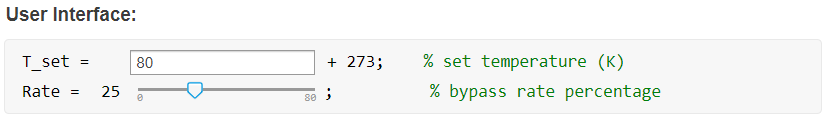
\includegraphics[width=12cm]{images/userinterface.png}
    \caption{Matlab user interface.}
    \label{fig:user}
\end{figure}

In Figure \ref{fig:resistor}, the heat transfer from the resistor to oil is shown in a simplified manner. It is entered into Simulink as shown in Figure \ref{fig:resistorsim}.

\begin{figure}[h]
    \begin{minipage}{.5\textwidth}
        \centering
        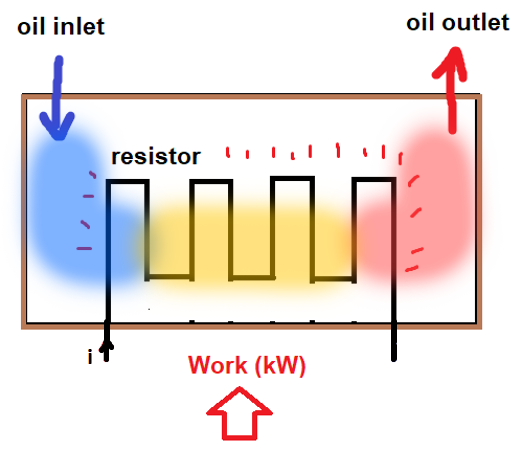
\includegraphics[width=6cm]{images/resistor.png}
        \captionof{figure}{Resistor schematic.}
        \label{fig:resistor}
    \end{minipage}
    \begin{minipage}{.4\textwidth}
        \centering
        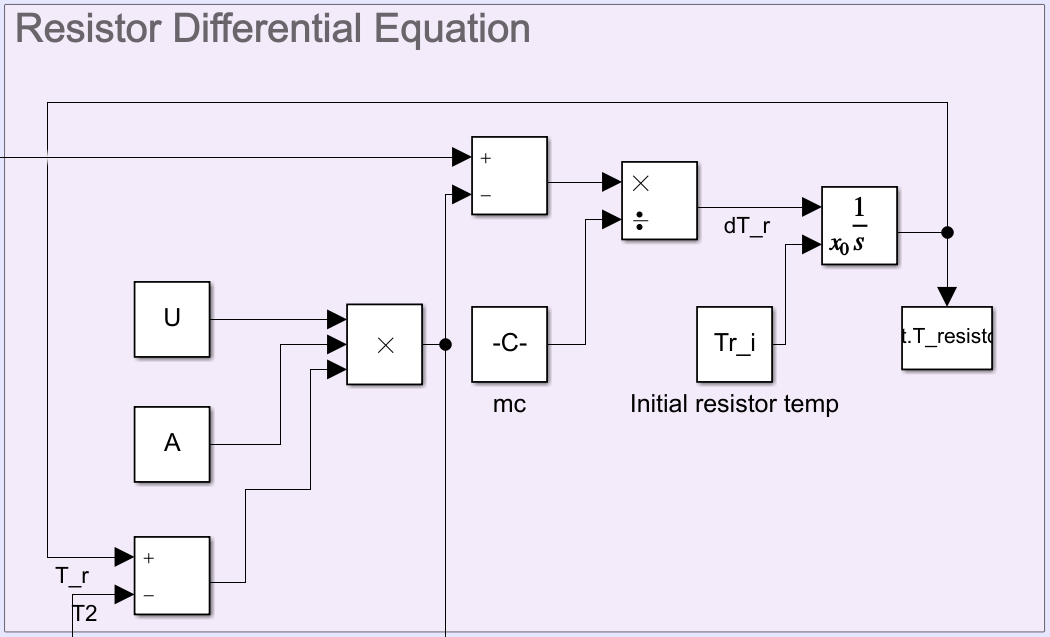
\includegraphics[width=7cm]{images/resistorsim.png}
        \captionof{figure}{Resistor Simulink model.}
        \label{fig:resistorsim}
    \end{minipage}
\end{figure}

\par
Figure \ref{fig:control} shows the temperature variations of the resistor, oil, and on-off status of the controller as input work. 

\par
Also, in Figure \ref{fig:energyflow}, the energy flow in this system can be seen clearly. Electrical energy is transformed into internal energy in the resistor. Then the oil's temperature is increased by the resistor, and finally, in the evaporator, R134A is heated up.


All parameters are found to solve for the temperature at the heater exit except for the resistor's heat transfer coefficient, surface area, mass, and specific heat. These four parameters are treated as two free variables as $UA$ and $m_{r}c_{r}$. These two variables are optimized to give minimum root-mean-square error in Section \ref{training}.

\begin{figure}[H]
    \centering
    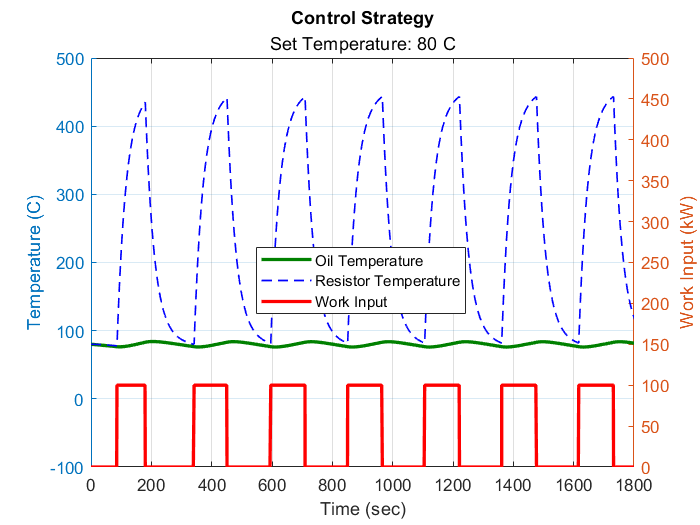
\includegraphics[width=11cm]{images/control_strategy.png}
    \caption{Temperature variations with control strategy.}
    \label{fig:control}
\end{figure}

\begin{figure}[H]
    \centering
    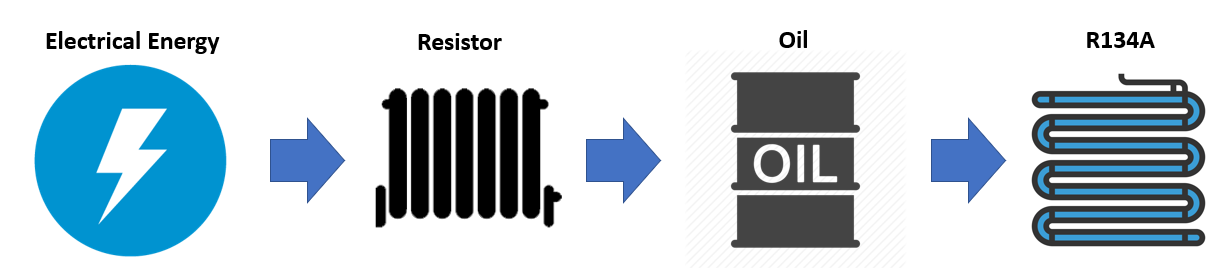
\includegraphics[width=14cm]{images/energyflow.png}
    \caption{Energy flow through the system.}
    \label{fig:energyflow}
\end{figure}

\subsection{Evaporator}
The evaporator model is very similar to the heater model in many respects. Parameters for the evaporator are provided in Table \ref{tab:evaporator}.

\begin{table}[h]
    \centering
    \caption{Evaporator parameters.}
    \label{tab:evaporator}
    \begin{tabular}{|c|c|c|}
        \hline
        \textbf{Symbol} & \textbf{Property}                         & \textbf{Unit} \\
        \hline
        $T_{4}$         & Oil temperature in evaporator             & Kelvin \\
        $m_{4}$         & Oil mass in evaporator                    & kg \\
        $c_{4}$         & Oil's specific heat in evaporator         & kJ/kg*K \\
        $Q_{e}$         & Heat transferred to R134A from oil        & kJ \\
        $\dot{m_{3}}$   & Oil mass flow rate at evaporator entrance & kg/s \\
        $\dot{m_{4}}$   & Oil mass flow rate at evaporator exit     & kg/s \\
        $h_{3}$         & Oil enthalpy at evaporator entrance       & kJ/kg \\
        $h_{4}$         & Oil enthalpy at evaporator exit           & kJ/kg \\
        \hline
    \end{tabular}
\end{table}

The governing differential equation for the evaporator, which is solved to obtain the temperature at the exit of the evaporator, is given in Equation \ref{eqn:evaporator}.

\begin{equation}
    \label{eqn:evaporator}
    \frac{dT_{4}}{dt} = \frac{1}{m_{4}c_{4}}(Q_{e} + \dot{m_{3}}h_{3} - \dot{m_{4}}h_{4})
\end{equation}

In this equation, mass, specific heat, mass flow rates, and enthalpy values are found with the same method provided for the heater using lookup tables. The mass here represents the oil mass inside the evaporator. This mass can be calculated by calculating the volume of the oil inside the evaporator. According to Ertugrul's thesis \cite{altun}, the plates of the evaporator have sinusoidal shapes having a perimeter of 7,64 mm, the area of a sinus wave is $A = 4 mm^2$ per wave, and the heat transfer area is $7.4 m^2$. This means that the total height of the sinusoidal-shaped heat transfer areas must be $h = \frac{7.4 m^2}{7,64 mm}$, and the oil volume inside the evaporator can be calculated as $V = h A = \frac{7.4 m^2}{7,64 mm} 4 mm^2 = 0.387 x 10^{-3} m^3$.

\par
Heat transfer between R134A and oil ($Q_{e}$) is found using experimental values. The temperature of the oil at the inlet and outlet of the evaporator is known. Combining this knowledge with the mass flow rate of the oil, Equation \ref{eqn:Qe} is obtained, which gives the experimental heat transfer amounts for each temperature.

\begin{equation}
    \label{eqn:Qe}
    Q_{e} = \dot{m}c(T_{4} - T_{3})
\end{equation}

Heat transfer value ($Q_{e}$) needs to be updated every second according to the current temperature and for all possible temperature ranges. To do that, experimental values are plotted against temperature, and four different curves are fitted to the plot for four regions. Then, the coefficients of these curves' equations are interpolated for unknown temperature values. This process is explained in Figure \ref{fig:curvefit}.

\begin{figure}[h]
    \centering
    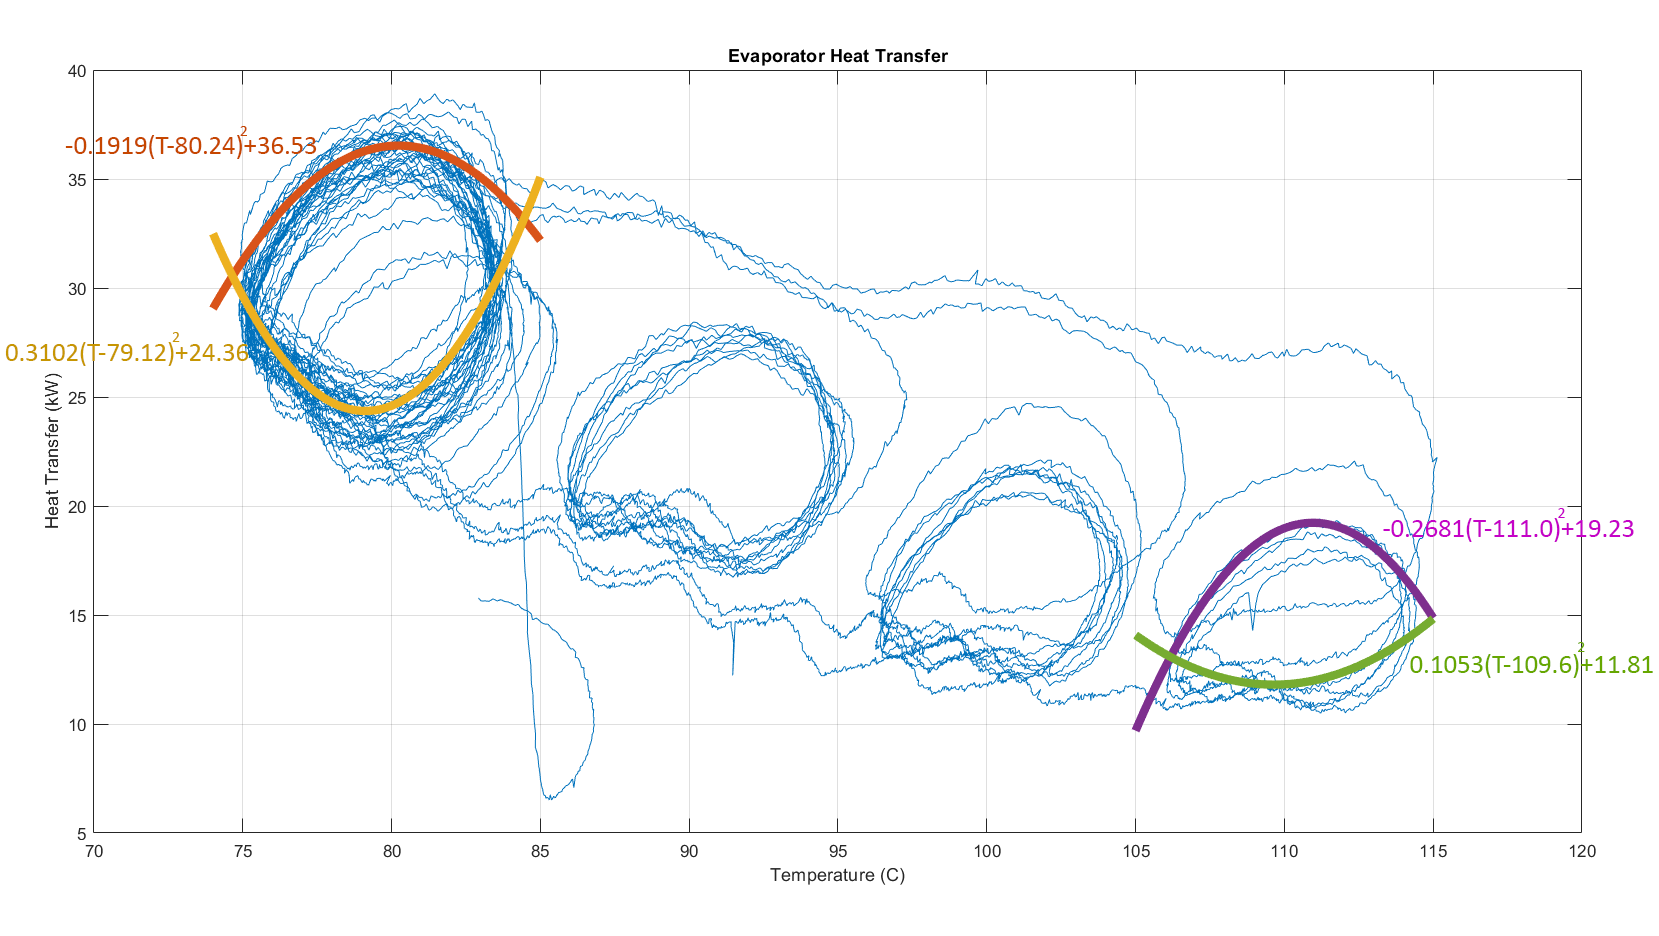
\includegraphics[width=16cm]{images/evaporator_fit.png}
    \caption{Evaporator heat transfer curve fitting to experimental data.}
    \label{fig:curvefit}
\end{figure}

Second-degree polynomials are fitted either in concave or convex format to represent the circular behavior of the data. General format of the polynomial is $Q_{e}(T) = a(T+b)^2+c$. Obtained coefficients are provided in Table \ref{tab:polyfit}.

\begin{table}[h]
    \centering
    \begin{tabular}{|c|c|c|c|}
        \hline
        Type                    & a & b & c \\
        \hline
        Concave, 80 $^\circ C$   & -0.1919 & -80.24 & 36.53 \\
        Concave, 110 $^\circ C$  & -0.2681 & -111.0 & 19.23 \\
        Convex, 80 $^\circ C$   & 0.3102  & -79.12 & 24.36 \\
        Convex, 110 $^\circ C$  & 0.1053  & -109.6 & 11.81 \\
        \hline
    \end{tabular}
    \caption{Coefficients of fitted polynomials.}
    \label{tab:polyfit}
\end{table}

\subsection{Tank}
The tank acts as a pressure stabilizer. The total oil volume in the system changes according to the temperature because temperature changes density. This change in volume is compensated in the tank. Parameters for the tank are provided in Table \ref{tab:tank}.

\begin{table}[h]
    \centering
    \caption{Tank parameters.}
    \label{tab:tank}
    \begin{tabular}{|c|c|c|}
        \hline
        \textbf{Symbol} & \textbf{Property}                         & \textbf{Unit} \\
        \hline
        $T_{1}$         & Oil temperature in tank             & Kelvin \\
        $m_{1}$         & Oil mass in tank                    & kg \\
        $c_{1}$         & Oil's specific heat in tank         & kJ/kg*K \\
        $Q_{loss}$      & Total heat loss in the system       & kJ \\
        $\dot{m_{4}}$   & Oil mass flow rate at tank entrance & kg/s \\
        $\dot{m_{1}}$   & Oil mass flow rate at tank exit     & kg/s \\
        $h_{4}$         & Oil enthalpy at tank entrance       & kJ/kg \\
        $h_{1}$         & Oil enthalpy at tank exit           & kJ/kg \\
        \hline
    \end{tabular}
\end{table}

Tank is also governed by a similar differential equation provided in Equation \ref{eqn:tank}. 

\begin{equation}
    \label{eqn:tank}
    \frac{dT_{1}}{dt} = \frac{1}{m_{1}c_{1}}(Q_{loss} + \dot{m_{4}}h_{4} - \dot{m_{1}}h_{1})
\end{equation}

Heat loss ($Q_{e}$) represents the total heat loss in the system. Heat loss normally occurs in every part, such as pipes, pump, heater, and evaporator, but it is introduced in the tank for ease of solution. It is also another free variable since it is unknown. 

\section{Training}\label{training}
There are three free variables:
\begin{itemize}
    \item Resistor's overall heat transfer coefficient and surface area: $UA$
    \item Resistor's mass and specific heat: $m_{r}c_{r}$
    \item Total heat loss from the system: $Q_{loss}$
\end{itemize}

Before training the model, experimental data is divided into two parts: one for training and the other for validation. This is because, for the reliability of validation, training data needs to be different from the validation data. This separation is shown in Figure \ref{fig:experimentaldata}.

\begin{figure}[h]
    \centering
    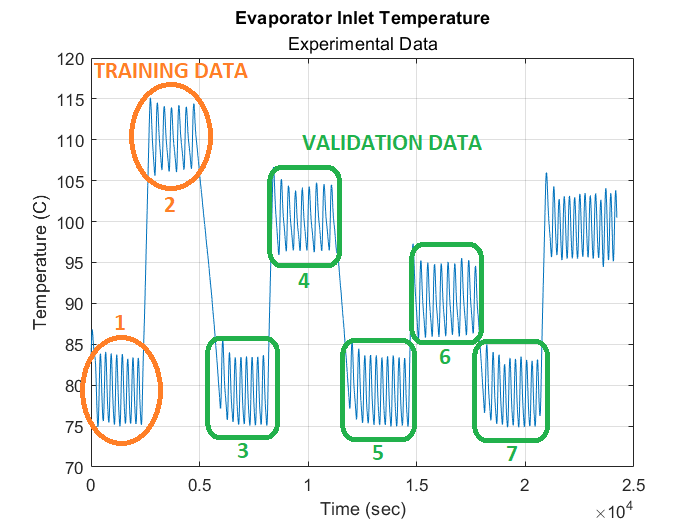
\includegraphics[width=13cm]{images/experimental-data.png}
    \caption{Experimental oil temperature data at evaporator inlet.}
    \label{fig:experimentaldata}
\end{figure}

As seen in Figure \ref{fig:experimentaldata}, in the first section of the experiment temperature is set to 80 $^\circ$C. Then, it is set to 110 $^\circ$C, which is the maximum temperature in the experiment. Oscillation frequency and amplitude change when set temperature is changed. Two far ends are selected as training data to get the nature of these oscillation frequency and amplitude changes.
\par
Many tests are carried out to determine the variables. Comparison plots are created, and RMSE values are calculated for each test. Plots are investigated to prevent under-fitting and over-fitting behaviors because if only the RMSE value is looked at, wrong results may be obtained.
\par
Variables to be determined can be divided into two categories. $UA$ and $m_{r}c_{r}$ are almost constant for all temperature values, and they are assumed as constant. Besides, $Q_{loss}$ significantly changes with the varying temperature, and it accounts for the previously mentioned oscillation frequency and amplitude change with the temperature. That's why at first, two variables $UA$ and $m_{r}c_{r}$ are determined from the test results. Then, the last variable $Q_{loss}$ fits the data both at higher temperatures and lower temperatures.
\par
Final values of the variables:
\begin{itemize}
    \item $UA = 0.27$ \textit{W/K}
    \item $m_{r}c_{r} = 8$ \textit{W/K}
    \item $Q_{loss} = -7.4074*10^{-06}*(T_{set}-110)^4 - 8$ \textit{W}
\end{itemize}

The final version of the plots that are used in the optimization of the variables is provided in Figures \ref{fig:test1} and \ref{fig:test2}.

\begin{figure}[h]
    \begin{minipage}{.5\textwidth}
        \centering
        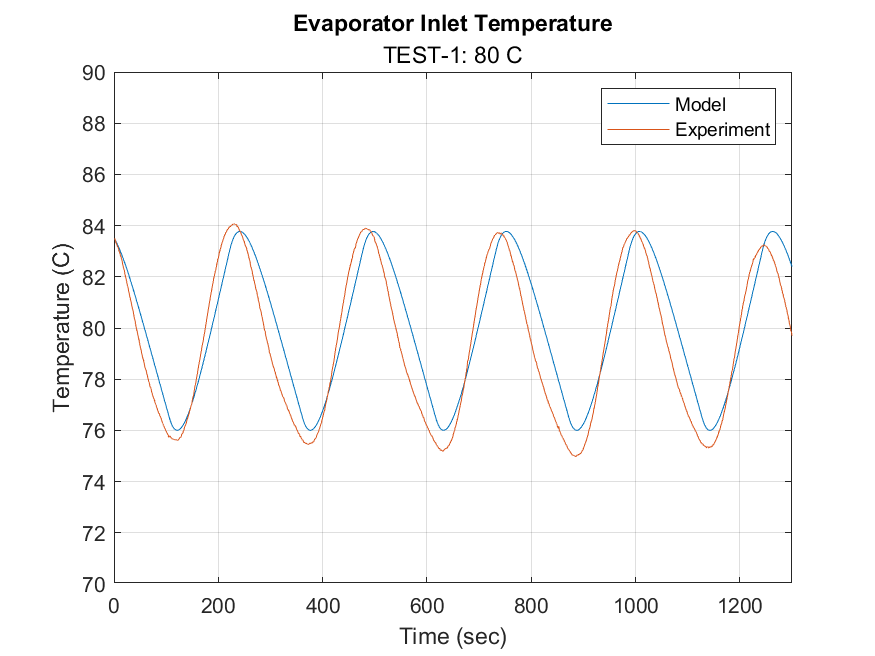
\includegraphics[width=8cm]{images/TEST-1.png}
        \captionof{figure}{Test-1.}
        \label{fig:test1}
    \end{minipage}
    \begin{minipage}{.4\textwidth}
        \centering
        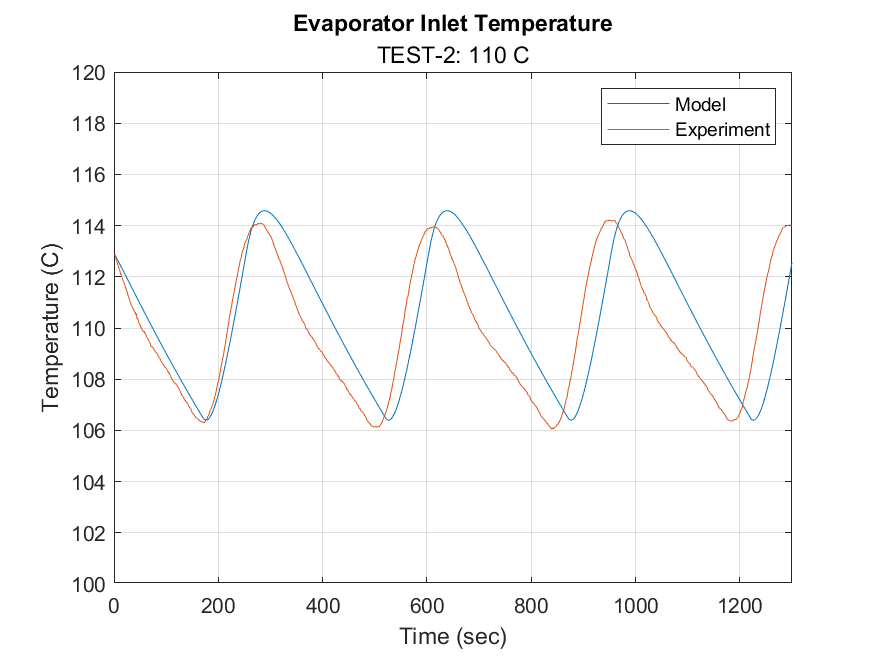
\includegraphics[width=8cm]{images/TEST-2.png}
        \captionof{figure}{Test-2.}
        \label{fig:test2}
    \end{minipage}
\end{figure}


\section{Proposed Solution}

\begin{figure}[H]
    \centering
    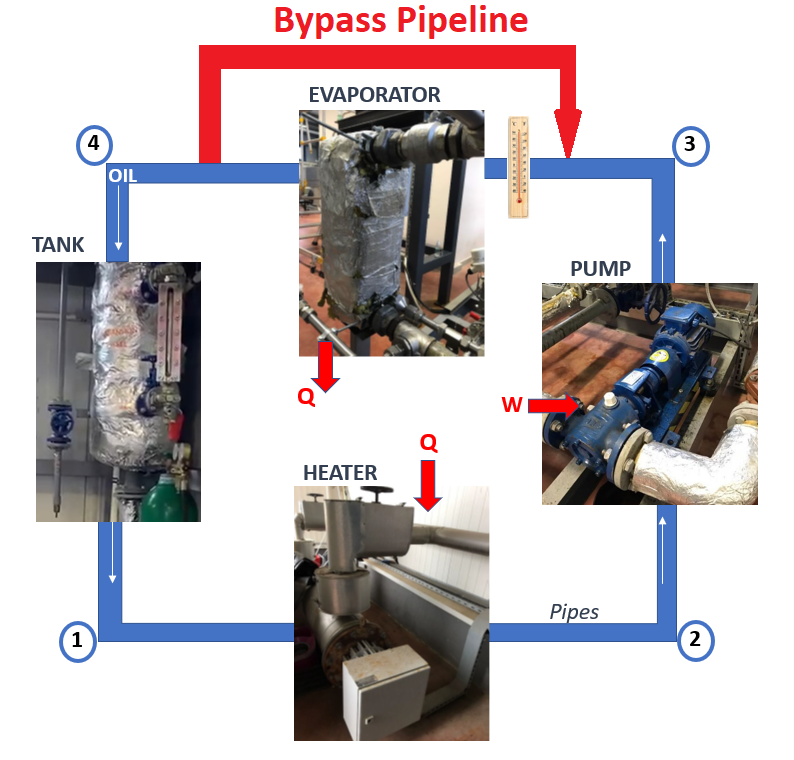
\includegraphics[width=10cm]{images/cycle_v2.png}
    \caption{Oil cycle with suggested method.}
    \label{fig:cycle_v2}
\end{figure}

The main goal of this project is to reduce the oil's temperature oscillations in the evaporator by applying mechanical solutions. A lower oscillation portion of the oil can be mixed with the mainstream oil just before the evaporator inlet. In Figure \ref{fig:cycle_v2}, our suggested method is implemented on the oil cycle.


According to the investigations of the experimental data, it is found that the oil's temperature oscillations are lower at the evaporator exit. Also, there already exists a bypass line between the inlet and exit of the evaporator. Thus, the proposed solution is feeding back the exiting oil to the inlet of the evaporator via this bypass line. This method is implemented in Simulink as seen in Figure \ref{fig:oldandnew}.

\bigskip

\begin{figure}[H]
    \centering
    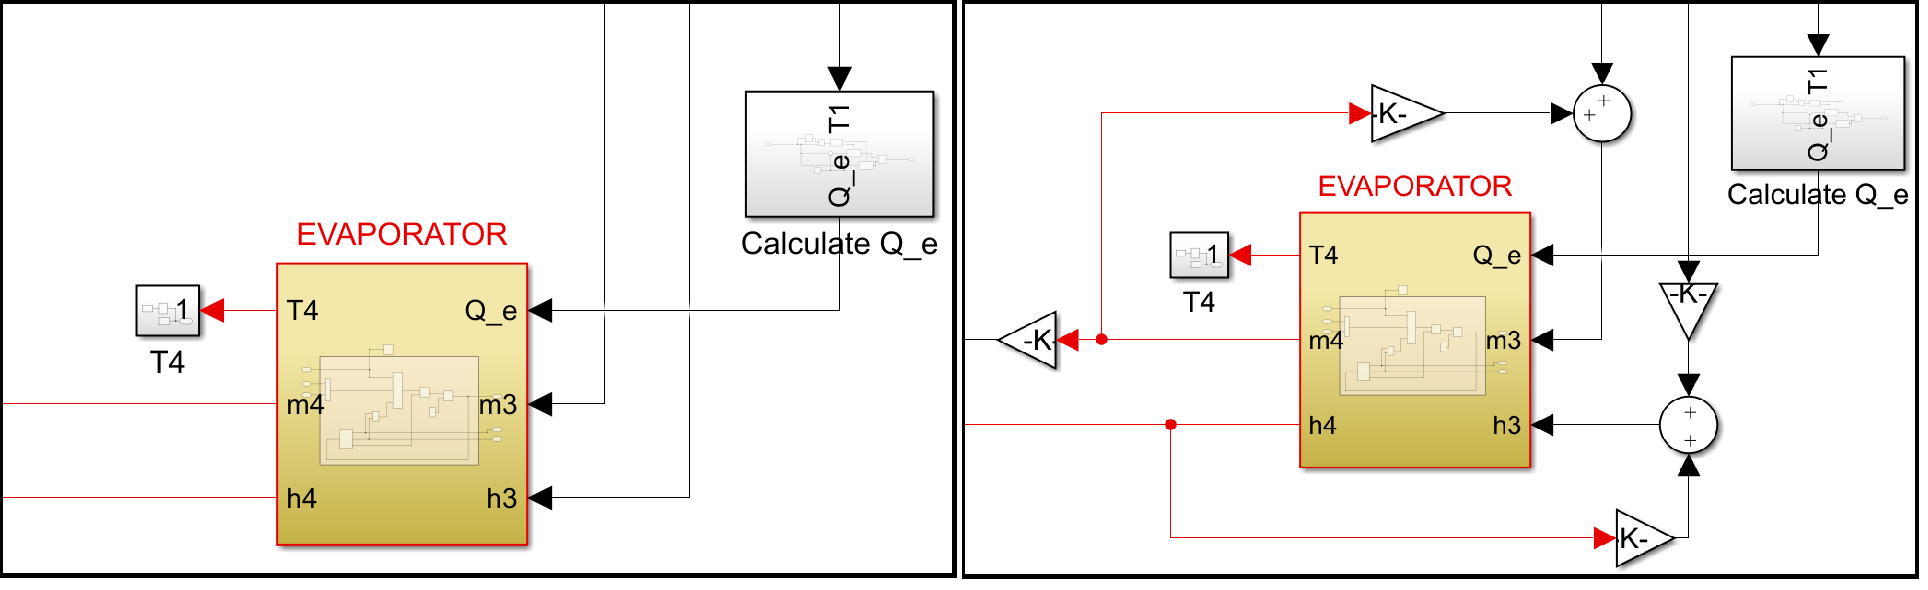
\includegraphics[width=14cm]{images/oldandnew.png}
    \caption{Evaporator model before and after the proposed solution is implemented.}
    \label{fig:oldandnew}
\end{figure}